\documentclass[compress, aspectratio=54]{beamer}
%\documentclass[notes=show]{beamer}
%\documentclass[xcolor=dvipsnames]{beamer}
\usepackage[export]{adjustbox}
\usepackage{sidecap}
\usepackage{subfig}
\usepackage{amssymb}
\usepackage{latexsym}
\usepackage{amsfonts}
\usepackage{amsmath}
\usepackage[absolute,overlay]{textpos}
\usepackage[english]{babel}
\usepackage[latin1]{inputenc}
\usepackage{subfig}
%\usepackage{times}
\usepackage[T1]{fontenc}
\usepackage{tabularx}
\newcolumntype{Y}{>{\small\raggedright\arraybackslash}X}
\usepackage{graphicx}
\usepackage{bigstrut}
\usepackage{bbm}
\usepackage{mathrsfs}
\usepackage{epsfig}
\usepackage{array}
%\usepackage{natbib}
\usepackage{hyperref}
\usepackage{caption}
\usepackage{comment}

\mode<presentation> {
%\usetheme[left,width=1.7cm]{Berkeley}
%\usetheme{default}
\usetheme{Boadilla}
  \usecolortheme[RGB={103,102,204}]{structure}
%\usecolortheme{dove}
  \useoutertheme{infolines}
  \setbeamercovered{transparent}
 }

%\usepackage[utf8]{inputenc}

% Default fixed font does not support bold face
\DeclareFixedFont{\ttb}{T1}{txtt}{bx}{n}{12} % for bold
\DeclareFixedFont{\ttm}{T1}{txtt}{m}{n}{12}  % for normal

% Custom colors
\usepackage{color}
\definecolor{deepblue}{rgb}{0,0,0.5}
\definecolor{deepred}{rgb}{0.6,0,0}
\definecolor{deepgreen}{rgb}{0,0.5,0}

\usepackage{listings}

% Python style for highlighting
\newcommand\pythonstyle{\lstset{
language=Python,
basicstyle=\ttm,
otherkeywords={self},             % Add keywords here
keywordstyle=\ttb\color{deepblue},
emph={MyClass,__init__},          % Custom highlighting
emphstyle=\ttb\color{deepred},    % Custom highlighting style
stringstyle=\color{deepgreen},
frame=tb,                         % Any extra options here
showstringspaces=false            % 
}}


% Python environment
\lstnewenvironment{python}[1][]
{
\pythonstyle
\lstset{#1}
}
{}

% Python for external files
\newcommand\pythonexternal[2][]{{
\pythonstyle
\lstinputlisting[#1]{#2}}}

% Python for inline
\newcommand\pythoninline[1]{{\pythonstyle\lstinline!#1!}}
%\renewcommand{\familydefault}{cmss}
%\renewcommand{\mathrm}{\mathsf}
%\renewcommand{\textrm}{\textsf}
\usefonttheme{serif}
\newcommand{\X}{{\mathbf{X}}}
\newcommand{\x}{{\mathbf{x}}}
\newcommand{\E}{\mathsf{E}}
\newcommand{\V}{\mathsf{Var}}

\DeclareGraphicsExtensions{.jpg,.pdf,.mps,.png}

\setbeamercolor{bibliography entry title}{fg=black}
\setbeamercolor{bibliography entry author}{fg=black}
\setbeamercolor{subsection in toc}{fg=structure}
\setbeamercolor{palette primary}{bg=structure, fg=white}
%\setbeamercolor{palette secondary}{bg=structure, fg=black}
%\setbeamercolor{palette tertiary}{bg=structure, fg=black}
\setbeamercolor{caption name}{fg=black} \setbeamersize{text margin
left=.8cm} \setbeamersize{text margin right=1cm}
\hypersetup{linkbordercolor={1 0 0}} \setbeamertemplate{navigation
symbols}{} \setbeamertemplate{headline}[default]

\setbeamertemplate{enumerate items}[default]

\newcounter{transfct}
\newcounter{begbs}
\newcounter{endbs}


\title[Introduction]{Text Analysis and Visualization with Python}

\author[Arieda Mu\c co]{Arieda Mu\c co}
\institute[CEU]{Central European University}

\AtBeginSection[] {
  \begin{frame}<handout:0>
    \frametitle{TOC}
    \tableofcontents[currentsection]
  \end{frame}
}

\date{}

\pgfdeclareimage[height=.7cm]{logo}{rgs2}
\logo{\pgfuseimage{logo}}
\begin{document}
\captionsetup[subfigure]{labelformat=empty}

\frame{\titlepage}

%%%%%%%%%%%%%%%%%%%%%%%%%%%%%%%%%%%%%%%%%%%


\begin{frame}
\frametitle{Information}
\begin{itemize}
\item My research focuses covers two main areas: Political and Development Economics. In my research, I deal with tons of data and (lots of) text data. That's why this course.
\item Introduce yourself. What are your expectations? Why are you here? What kind of text/data you are currently using or plan to use? 
\end{itemize}
\end{frame}
%----------------------------------------------------------------------------%

\begin{frame}
\frametitle{Plan for this course}
\begin{itemize}
\item Introduction to Python foundations
\item Data collection and processing, word counts
\item Supervised text methods, classification
\item Unsupervised text methods, topic models and clustering
\item Data Visualization
\end{itemize}
\end{frame}
%----------------------------------------------------------------------------%


\begin{frame}
\frametitle{Grading}
Final assessment will consist of the following:
\begin{itemize}
\item \textbf{Quizzes in Class} (20\% of final grade)
\item \textbf{Problem Sets} (40\% of final grade)
\item \textbf{Individual Project}  (40\% of final grade)
\end{itemize}
\end{frame}

%----------------------------------------------------------------------------%

%----------------------------------------------------------------------------%


\begin{frame}
\frametitle{Deadlines}

\begin{itemize}
\item Past deadline submissions do not get graded
\item Email for meetings, questions etc 
\item Emails/Questions: You will get a reply if you send an email but send it 24 hours before a deadline (no response otherwise)
\item Slack will be our communication tool for this course
\begin{itemize}
\item Post questions and answers in respective channels
\item Keep a close eye on channels on quizzes and assignments
\item Make sure you reply in thread when needed.
\end{itemize}
\item We strongly encourage peer learning. Feel free to post in the Slack channel if you think some information is of common interest
\end{itemize}

\end{frame}

%----------------------------------------------------------------------------%
\begin{frame}
\frametitle{Rules}
\begin{itemize}
\item Ask questions and feel free to google
\begin{itemize}
\item Don't feel bad about this. Even software developers spend a lot of their coding time googling programming related questions
\item Important to know how to read error messages
\begin{itemize}

\item or google them
\end{itemize}
\item Stack Overflow is a programmer's best friend
\end{itemize}
\end{itemize}
\end{frame}

%----------------------------------------------------------------------------%

\begin{frame}
\begin{figure}

\includegraphics[width=0.6\linewidth ]{Figures/stack-overflow.jpeg}
\end{figure}

\end{frame}

%----------------------------------------------------------------------------%
\begin{frame}
\frametitle{Recommended Material}
\begin{itemize}
\item \href{https://www.codecademy.com/catalog/language/python}{\color{ blue}{Codecademy}} is the place to start
\item \href{https://automatetheboringstuff.com/}{\color{ blue}{Automate the Boring Stuff with Python}} and \href{https://realpython.com/}{\color{ blue}{The Real Python}} are great sources
%
\item \href{https://nlp.stanford.edu/IR-book/information-retrieval-book.html}{\color{ blue}{Introduction to Information Retrieval}} by Christopher D. Manning, Prabhakar Raghavan and Hinrich Schutze

\item  Speech and Language Processing by Dan Jurafsky and James H. Martin
\item  Introduction to Machine Learning with Python: A Guide for Data Scientists by Sarah Guido, and Andreas Muller
\end{itemize}
\end{frame}

%----------------------------------------------------------------------------%
\begin{frame}
\frametitle{Text and Social Sciences}
 Before 2000's social scientists avoided studying texts/speech. Why?
\begin{itemize}
\item Time Consuming
\item Not generalizable (each new data set...new coding scheme)
\item Difficult to store/search
\item Idiosyncratic to coders/researcher
\item Statistical methods/algorithms, computationally intensive
\item Hard to find

\end{itemize}
\end{frame}

%----------------------------------------------------------------------------%


\begin{frame}
\frametitle{Text and Social Sciences}
Massive collections of texts are increasingly used as a data source in social
science:
\begin{itemize}
\item Congressional speeches, press releases, newsletters,...
\item Facebook posts, tweets, emails, cell phone records, ...
\item Newspapers, magazines, news broadcasts, ...
\item Foreign news sources, treaties, sermons, ...

\end{itemize}
\end{frame}

%----------------------------------------------------------------------------%



\begin{frame}
\frametitle{Why?}
Massive increase in availability of unstructured text
\begin{itemize}
\item Cheap storage: 1956: $\$10,000 $ megabyte. $2019: <<<<< \$0.0001$ per megabyte
\item Explosion in methods and programs to analyze texts

\begin{itemize}
\item Generalizable: one method can be used across many methods and to
unify collections of texts
\item Systematic: parameters/statistics demonstrate how models make
coding decisions
\item Cheap: easily applied to many new collections of texts, computing
power is inexpensive
\item Replicable: using the same text and method we reach the same conclusions
\end{itemize}
\item  Social life (politics, economic exchanges, social interactions)
occurs in texts
\end{itemize}
\begin{itemize}
\item Laws, Treaties, News, Campaigns, Petitions, Press Releases
\end{itemize}
\end{frame}

%----------------------------------------------------------------------------%


\begin{frame}
\frametitle{What to do with Text Data?}
Growth of a field called Computational Social Science
\begin{itemize}
\item Lots of interest across fields
\item Computer Science, Computational Linguistics, Education, Sociology,
Library and Information Science, Political Science, Communications,
Physics, and Economics
\item More and more text analysis and machine learning tools are getting incorporated into social scientific research

\end{itemize}
\end{frame}

%----------------------------------------------------------------------------%

\begin{frame}
\frametitle{What is Automated Content Analysis?}
\begin{itemize}

\item Blanket name for many things
\begin{itemize}
\item Exploration of text or other media
\item Using large text corpora as data
\item Data mining of large variable datasets
\end{itemize}

\item Automated: Computer assigned labels
\item Connected to many different literatures
\begin{itemize}
\item Machine learning
\item Natural Language Processing
\item Business Analytics
\item Visualization of Text
\item Data Mining
\item Statistics/Econometrics

\end{itemize}
\end{itemize}

\end{frame}

%----------------------------------------------------------------------------%

\begin{frame}
\frametitle{What Can Text Methods Do?}
Interpreting the meaning of a sentence or phrase. Analyzing a straw
of hay 
\begin{itemize}

\item Haystack metaphor: Improve Reading
\begin{itemize}
\item Humans: amazing (political theory, analysis of English
poetry)
\item Computers: struggle
\end{itemize}

\item Comparing, Organizing, and Classifying Texts. Organizing hay stack
\begin{itemize}
\item Humans: terrible. Tiny active memories
\item Computers: amazing (we'll discuss in this course)
\end{itemize}
\end{itemize}

What automated text methods don't do:
\begin{itemize}

\item Replace the need to read
\item Develop a single tool + evaluation for all tasks
\end{itemize}
\end{frame}

%----------------------------------------------------------------------------%

\begin{frame}
\frametitle{Why Python?}




\[\begin{array}{ccc}

\includegraphics[height=2cm]{Figures/trends_languages.png} &{\includegraphics[height=3cm]{Figures/Economist_Python3}}& {\includegraphics[height=3cm, width=3.5cm]{Figures/Economist_Python}} \\

  \end{array}
\]


\end{frame}
%----------------------------------------------------------------------------%


\begin{frame}
\frametitle{A bit about Python}
\begin{itemize}

\item Programming language intended for general purpose high-level language
\item Web development, scientific and numeric education, desktop graphical user interface, software development
\item Free and open source 
\item You can do everything that you can do in a programming language
\item Big community (Google, Youtube, Nasa...)
\item High readability (more than R or C)
\item Python was first released in early 1980
\begin{itemize}

\item Python 2 in 2000 and Python 3 in 2008
\end{itemize}
\end{itemize}

\end{frame}
%----------------------------------------------------------------------------%
%----------------------------------------------------------------------------%

\begin{frame}
\frametitle{Black Holes and Python}
\begin{figure}

\includegraphics[width=0.5\linewidth ]{Figures/black_hole.png}
\end{figure}

\end{frame}

%----------------------------------------------------------------------------%
\begin{frame}
\frametitle{Annoying things in Python}
\begin{itemize}

\item Python 3 is not backward compatible with Python 2
\begin{itemize}
\item In this course we will use Python 3. Python 2 is not supported anymore
\item If you are starting a new project, do so in Python 3
\end{itemize}

\item Pandas Library (more on this next time)
\begin{itemize}
\item But very useful 
\end{itemize}
\item + some minor things we'll cover throughout the course 
\begin{itemize}

\item example: split() vs join()
\begin{itemize}
\item sentence = "We will rock you!"

\item words = sentence.split(" ") but sentence = " ".join(words) (?)
\end{itemize}


\end{itemize}

\end{itemize}

\end{frame}
%----------------------------------------------------------------------------%
\begin{frame}
\frametitle{Purpose of the course}
\begin{itemize}

\item Text Analysis, Machine Learning, Data Visualization, and programming in Python are (mildly put) very broad topics, and we will not be able to cover many(!) things
\item Build strong foundations such that in the future you get confidence in starting to dig deeper into these topics
 
\end{itemize}

\end{frame}
%----------------------------------------------------------------------------%

%----------------------------------------------------------------------------%


\begin{frame}
\frametitle{Ada Lovelace a Pythonista}

 \begin{minipage}{0.5\textwidth}
 Ada was the first to recognize the full potential of a ``computing machine'' and one of the first computer programmers.
 \begin{itemize}

\item Basic concepts:
 \begin{itemize}
 \item Variables, subroutines, functions, methods, algorithm
 \item Programs as more than number crunching

  \end{itemize}

 \end{itemize}

 \end{minipage}%
\begin{minipage}{0.5\textwidth}
\begin{center}
    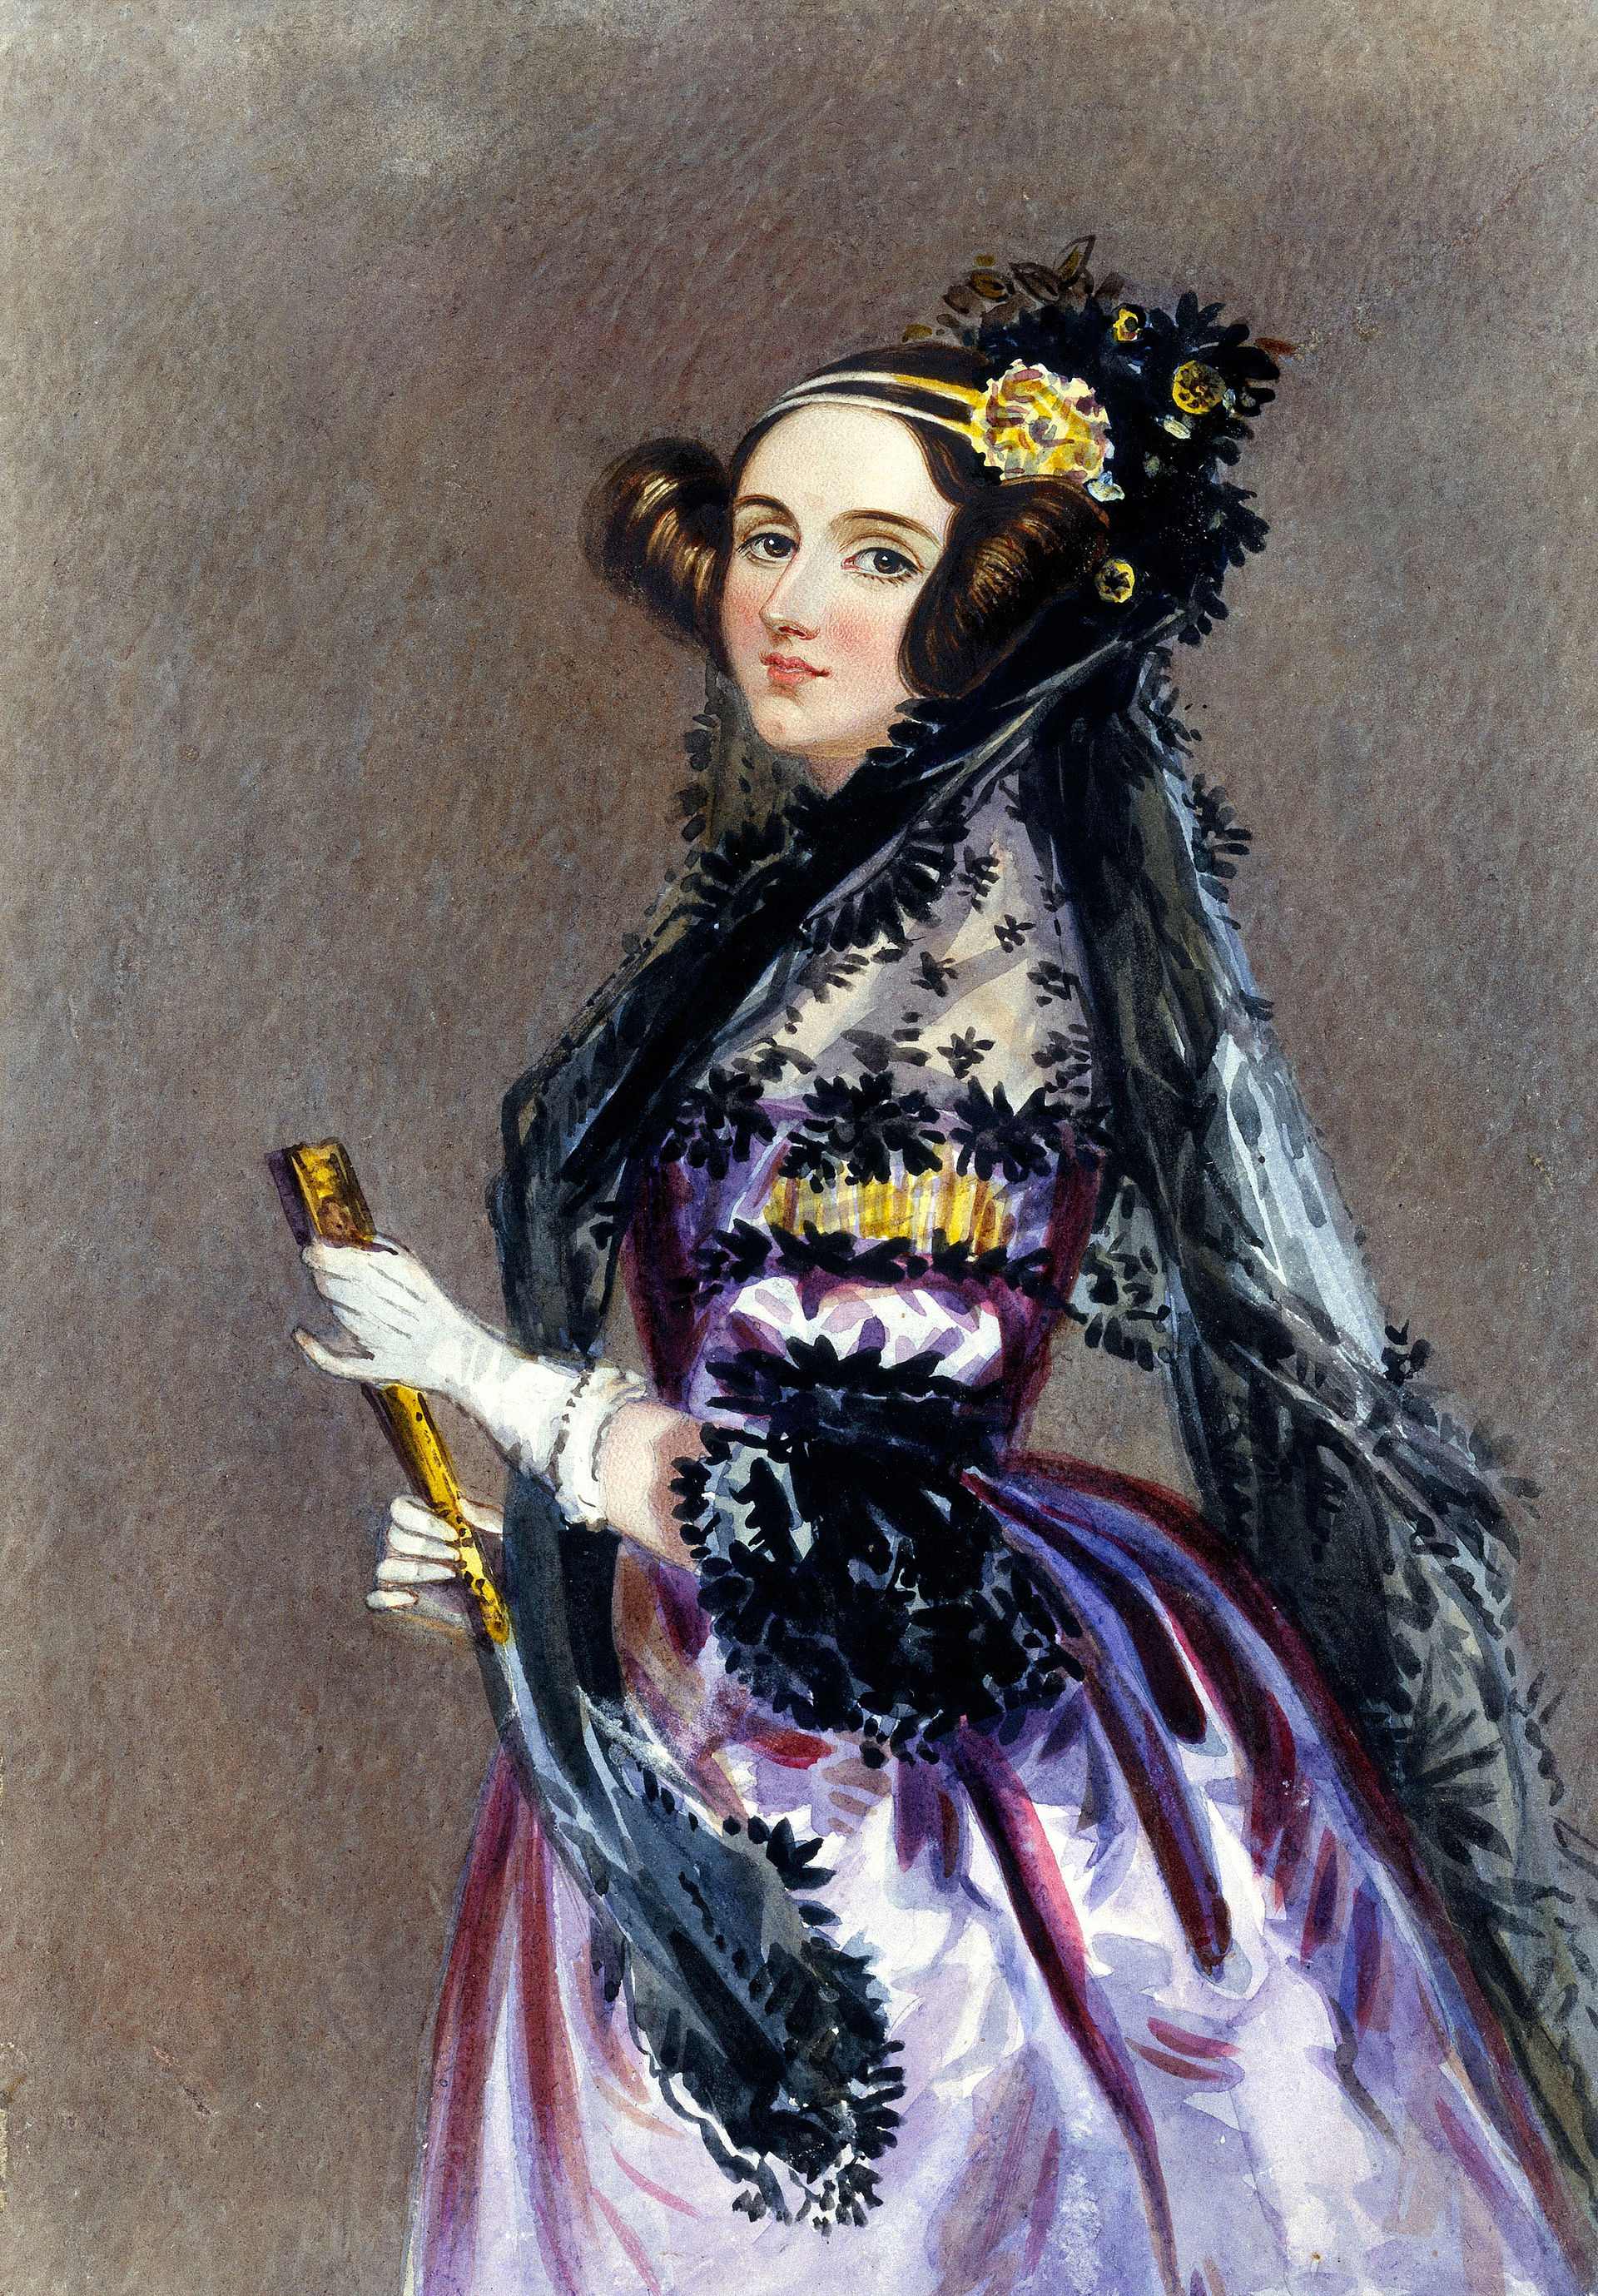
\includegraphics[width=0.6\textwidth]{Figures/Ada_Lovelace_portrait.jpg}
\end{center}
\end{minipage}
\end{frame}

%----------------------------------------------------------------------------%

\begin{frame}
\frametitle{Ada's basic concepts in Python}
\begin{itemize}

\item A variable
 \begin{itemize}

 \item radius = 7
 \end{itemize}

\item A constant
 \begin{itemize}

\item  PI = 3.14159
 \end{itemize}

 \item An algorithm
 \begin{itemize}

\item circumference = 2 * PI * radius
\end{itemize}
\end{itemize}

\end{frame}
%----------------------------------------------------------------------------%

\begin{frame}
\frametitle{Ada's basic concepts in Python}
\pythonexternal{ada.py}

\end{frame}

%----------------------------------------------------------------------------%
\begin{frame}
\begin{center}
\huge{Time to code!!!}
\end{center}

\end{frame}
\end{document}

